\chapter{Тепловая история, последнее рассеяние и первичный суп}

\lectureoverview{История расширения Вселенной — это также и тепловая история. Мы начнём с определения температуры через равновесие, а равновесия — через рассеяние. Фотонный газ приобретает планковский спектр, пока свободные заряды поддерживают его в тепловом равновесии; когда электроны связываются с протонами, излучение развязывается, но сохраняет форму спектра абсолютно чёрного тела, поскольку каждая длина волны растягивается вместе с масштабным фактором. Огромное отношение числа фотонов к числу частиц вещества затем объясняет, почему рекомбинация происходит при температуре, намного меньшей температуры ионизации водорода. Продолжая идти назад, мы проходим через последнее рассеяние, равенство вещества--излучения, равновесие электрон--позитронных пар и, наконец, небольшой избыток вещества--антивещества, переживающий аннигиляцию.}

\section{От подгонки модели к тепловой истории}

Космологическая модель задаётся, как минимум, эволюцией масштабного фактора и пространственной геометрией,
\begin{equation}
a(t),
\qquad
k\in\{+1,0,-1\}.
\end{equation}
Практический метод состоит в том, чтобы выбрать модель, вычислить её предсказания, сравнить их с данными и скорректировать параметры. Непосредственный вывод в обратную сторону, прямо из данных, возможен, но часто менее прозрачен.

Кривизну трудно определить по сравнительно близким источникам. Подобно тому как кривизна Земли даёт лишь малую поправку на короткой наземной базе, пространственная кривизна является слабым эффектом, когда космологическая база недостаточно велика. В этом есть и недостаток, и преимущество: обычные обзоры источников не позволяют точно определить \(k\), но умеренная неопределённость в \(k\) не мешает полезной реконструкции истории расширения.

Большую часть нагрузки несут два семейства наблюдаемых величин. Стандартные свечи дают яркость как функцию красного смещения, тогда как обзоры источников дают число объектов в интервале красного смещения. Получающиеся подгонки указывают на историю расширения со значительным вкладом энергии вакуума. Для точной информации о кривизне требуется гораздо более длинное геометрическое плечо, которое даёт космический микроволновый фон.

Теперь мы меняем вопрос. Вместо того чтобы спрашивать только о том, как эволюционирует \(a(t)\), мы спрашиваем, как эволюционирует температура Вселенной. Этот вопрос начинается с более элементарного: при каких условиях система вообще имеет температуру?

\section{Когда Вселенной можно приписать температуру}

Температура — свойство теплового равновесия. Совокупность частиц приходит к равновесию через столкновения, и эти столкновения должны действовать быстрее, чем меняется макроскопическая среда. В расширяющейся Вселенной существенным является сравнение
\begin{equation}
\tau_{\rm scatt}\ll H^{-1},
\label{eq:c07-equilibrium-condition}
\end{equation}
где \(\tau_{\rm scatt}\) — характерное время рассеяния, а \(H^{-1}\) — время расширения. Когда это неравенство нарушается, Вселенная меняется раньше, чем столкновения успевают восстановить равновесие.

Рассмотрим идеально отражающий ящик. Направим в него лазерный импульс, закроем отверстие и предположим, что в ящике содержатся только фотоны. Импульс будет отражаться бесконечно долго, но обычные низкоэнергетические фотоны рассеиваются друг на друге чрезвычайно слабо. Одно лишь отражение не перераспределяет их энергию в тепловой спектр. Поэтому фотонный газ не термализуется просто потому, что он заключён в ящике.

Свободные заряженные частицы меняют ситуацию. Электромагнитная волна ускоряет электрон; ускоренный заряд переизлучает, поэтому фотоны рассеиваются эффективно. При достаточном числе свободных электронов и протонов многократное рассеяние перераспределяет энергию между всеми тремя компонентами, пока они не образуют единый тепловой суп с общей температурой.

На больших масштабах Вселенная электрически нейтральна. В простейшем учёте,
\begin{equation}
n_{e^-}=n_p,
\label{eq:c07-neutrality}
\end{equation}
поскольку заряды электрона и протона равны по модулю и противоположны по знаку. Это уравнение выражает нейтральность; оно не объясняет, почему выполняется электрическая нейтральность и почему модули этих двух зарядов совпадают. Это более глубокие факты физики частиц.

Различие между плазмой и нейтральным газом имеет решающее значение. Свободные электроны эффективно рассеивают излучение. Как только электроны связываются с протонами, образуя нейтральный водород, преобладающие электрические поля на больших расстояниях компенсируются, и рассеяние становится намного менее эффективным. При малой плотности современной Вселенной нейтральное вещество не может привести фоновые фотоны к равновесию за время жизни Вселенной.

При достаточно высокой температуре энергичные столкновения многократно ионизуют водород и поддерживают заметную популяцию свободных зарядов. Электроны, протоны и фотоны тогда имеют общую температуру. По мере охлаждения системы атомы сохраняются, плотность свободных электронов резко падает, и общее равновесие теряется. Температуры, которые после этого приписывают веществу и излучению, не обязаны совпадать.

\begin{classroomqa}
\audiencequestion{Если температура микроволнового фона близка к \(3\,\mathrm{K}\), является ли это температурой всей Вселенной сегодня?}
\lecturerresponse{Нет. Фотонному спектру можно приписать температуру абсолютно чёрного тела, но современное вещество не находится в равновесии с этими фотонами. Разные компоненты имеют разные кинетические или эффективные температуры, так что сегодня не существует единой глобальной термодинамической температуры.}
\end{classroomqa}

\section{Тепловое излучение и квантовый перелом}

Поле излучения в равновесии содержит спектр длин волн и частот, связанных соотношением
\begin{equation}
\nu\lambda=c.
\end{equation}
Чтобы не путать яркость с плотностью энергии, пусть \(u_\nu(T)\) обозначает энергию на единицу объёма и на единицу частоты:
\begin{equation}
dE=u_\nu(T)\,dV\,d\nu.
\label{eq:c07-spectral-density}
\end{equation}
Следовательно, \(u_\nu\) имеет размерность энергии, делённой на объём и частоту.

Сама температура — это энергетический масштаб. Исторически сложившиеся единицы температуры скрывают этот факт, поэтому постоянная Больцмана задаёт перевод:
\begin{equation}
E_{\rm thermal}\sim k_B T.
\end{equation}
В естественных единицах можно положить \(k_B=1\), но сохранение этой константы позволяет явно различать кельвины и энергию.

До появления квантовой механики размерный анализ с использованием \(k_BT\), \(\nu\) и \(c\) даёт спектральную плотность энергии Рэлея--Джинса,
\begin{equation}
u_\nu^{\rm RJ}(T)=\frac{8\pi\nu^2}{c^3}k_BT.
\label{eq:c07-rayleigh-jeans}
\end{equation}
Численный коэффициент зависит от подсчёта электромагнитных мод, но существенное классическое поведение таково: \(u_\nu\propto T\nu^2\). Эта величина неограниченно растёт с увеличением частоты и потому предсказывает
\begin{equation}
\int_0^\infty u_\nu^{\rm RJ}\,d\nu=\infty.
\end{equation}
Этот невозможный результат и есть ультрафиолетовая катастрофа. Вместо этого измеренный спектр растёт, проходит через максимум и падает достаточно быстро, чтобы полная энергия оставалась конечной.

Постоянная Планка вводит недостающий квантовый масштаб. Для спектральной плотности энергии, определённой в уравнении~\eqref{eq:c07-spectral-density}, закон Планка имеет вид
\begin{equation}
u_\nu(T)
=
\frac{8\pi h\nu^3}{c^3}
\frac{1}{e^{h\nu/(k_BT)}-1}.
\label{eq:c07-planck}
\end{equation}
Показатель экспоненты зависит от безразмерного отношения
\begin{equation}
x=\frac{h\nu}{k_BT},
\end{equation}
поскольку \(E_\gamma=h\nu\) и \(k_BT\) обе величины являются энергиями.

При низкой частоте, \(x\ll1\), и
\begin{equation}
e^x-1=x+O(x^2).
\end{equation}
Подстановка в уравнение~\eqref{eq:c07-planck} даёт
\begin{align}
u_\nu(T)
&\simeq
\frac{8\pi h\nu^3}{c^3}
\frac{k_BT}{h\nu}
\\
&=
\frac{8\pi\nu^2}{c^3}k_BT,
\end{align}
так что классическая физика восстанавливается в своей надлежащей области низких частот. При высокой частоте, \(x\gg1\), экспонента доминирует и подавляет спектр. Переход происходит при
\begin{equation}
\frac{h\nu}{k_BT}\sim1.
\label{eq:c07-crossover}
\end{equation}
Это та точка, в которой квантовый перелом сменяет классический рост.

\begin{figure}[htbp]
\centering
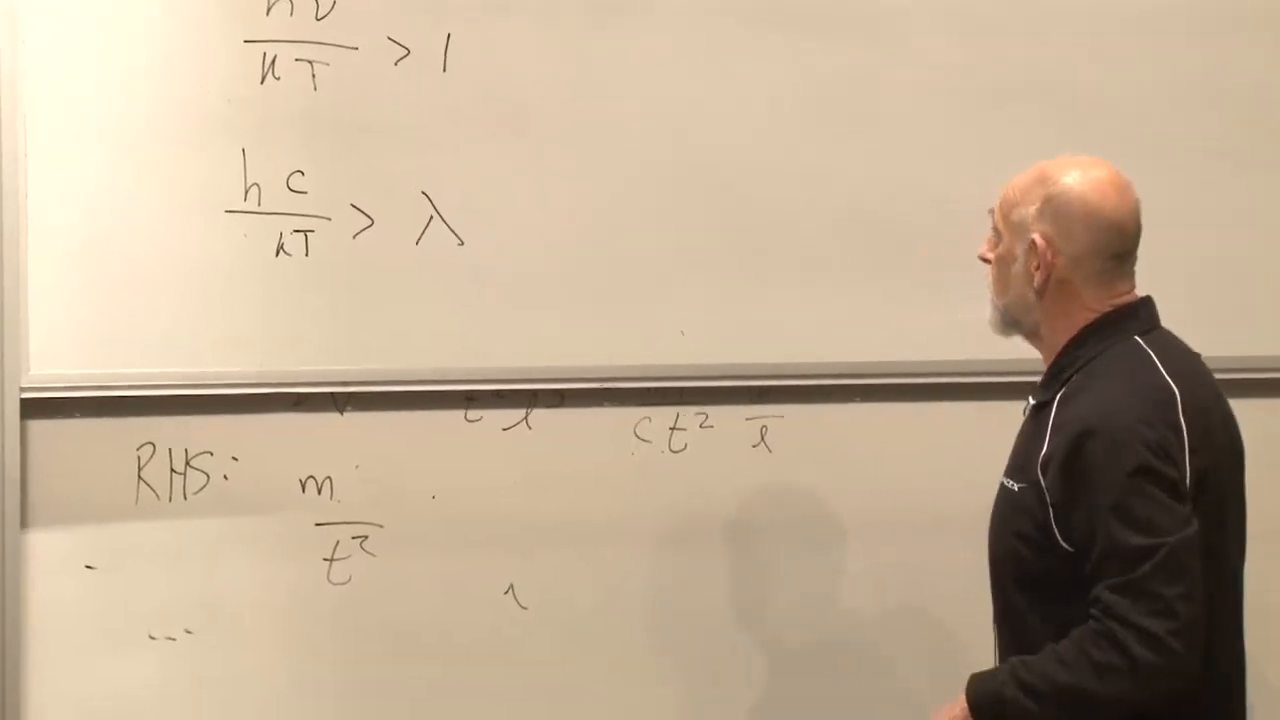
\includegraphics[width=0.82\textwidth]{lecture_07_figure_02.png}
\caption{Тепловой переход на доске. Обрезанное верхнее выражение имеет вид \(h\nu/(kT)>1\), а хорошо видимое нижнее выражение — \(hc/(kT)>\lambda\). Слабые следы на нижней доске не используются как подтверждение уравнения.}
\label{fig:c07-thermal-board}
\lectureframe{00:44:42.840}
\end{figure}

Используя \(\nu=c/\lambda\), этот переход задаёт тепловую длину волны по порядку величины,
\begin{equation}
\boxed{\lambda_{\rm th}\sim\frac{hc}{k_BT}}.
\label{eq:c07-thermal-wavelength}
\end{equation}
Более короткие длины волн лежат в экспоненциально подавленном хвосте; основная часть мощности приходится на длины волн этого порядка, с точностью до численного коэффициента, зависящего от того, изображён ли спектр на единицу частоты или на единицу длины волны.

\begin{classroomqa}
\audiencequestion{Получил ли Планк этот спектр из использованной здесь модели электрон--протонной плазмы?}
\lecturerresponse{Нет. Он объединил эмпирическую спектральную информацию с законом смещения Вина, который уже показывал, что длина волны в максимуме меняется обратно пропорционально температуре. Это масштабирование выявило новую постоянную \(h\). Планк связал результат с осцилляторами в материальных стенках, тогда как полная квантовая интерпретация поля излучения появилась позже. \lecturetimestamp{00:37:06--00:39:25}}
\end{classroomqa}

\begin{classroomqa}
\audiencequestion{Почему при размерностной проверке, по-видимому, потерялась одна степень \(c\)?}
\lecturerresponse{Величина, сначала названная интенсивностью, была определена как энергия на единицу объёма и на единицу частоты, тогда как знакомая формула с \(2h\nu^3/c^2\) — это спектральная яркость на единицу площади и телесного угла. Спектральная плотность энергии содержит \(c^{-3}\) и угловой множитель, как в уравнении~\eqref{eq:c07-planck}. Эта поправка меняет соглашение о нормировке, а не безразмерное отношение \(h\nu/(k_BT)\) и не тепловую длину волны. \lecturetimestamp{00:39:33--00:44:51}}
\end{classroomqa}

Если не считать нормировки, спектр Планка имеет универсальную форму. Уравнение~\eqref{eq:c07-planck} можно записать
\begin{equation}
u_\nu(T)=T^3\,F\!\left(\frac{\nu}{T}\right),
\label{eq:c07-scaling-form}
\end{equation}
поглотив константы в \(F\). Увеличение \(T\) перемасштабирует ось частот и общую высоту; вновь появляется одна и та же безразмерная кривая. В терминах длины волны повышение температуры сжимает спектр к более коротким длинам волн.

\begin{figure}[htbp]
\centering
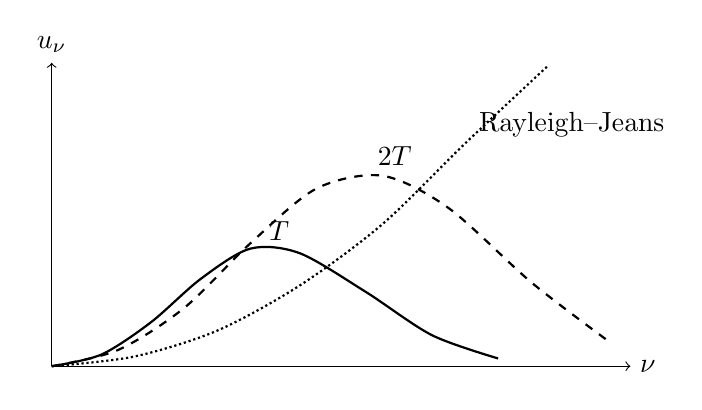
\begin{tikzpicture}[x=1.05cm,y=0.82cm]
\draw[->] (0,0)--(7.0,0) node[right] {\(\nu\)};
\draw[->] (0,0)--(0,4.7) node[above] {\(u_\nu\)};
\draw[densely dotted,thick] plot[smooth] coordinates
  {(0,0) (1,0.15) (2,0.55) (3,1.25) (4,2.20) (5,3.45) (6,4.65)};
\draw[thick] plot[smooth] coordinates
  {(0,0) (0.6,0.18) (1.2,0.68) (1.8,1.35) (2.4,1.82) (3.0,1.75) (3.8,1.15) (4.6,0.48) (5.4,0.12)};
\draw[thick,dashed] plot[smooth] coordinates
  {(0,0) (0.8,0.25) (1.6,0.90) (2.4,1.90) (3.2,2.75) (4.0,2.95) (4.8,2.45) (5.8,1.30) (6.7,0.42)};
\node[anchor=west] at (5.05,3.75) {Rayleigh--Jeans};
\node at (2.75,2.10) {\(T\)};
\node at (4.15,3.25) {\(2T\)};
\end{tikzpicture}
\caption{Классический спектр неограниченно возрастает, тогда как спектры Планка проходят через максимум. Повышение температуры смещает характерную частоту в сторону больших значений и сохраняет безразмерную форму.}
\label{fig:c07-planck-redraw}
\end{figure}

Подавляющее большинство фотонов в нынешней Вселенной принадлежит микроволновому фону и имеет характерную длину волны порядка миллиметра. Уравнение~\eqref{eq:c07-thermal-wavelength} сопоставляет этой длине волны температуру в несколько кельвинов, которую здесь по обыкновению округляют до \(3\,\mathrm{K}\). По одной лишь длине волны можно было бы получить только грубое соответствие. Более веское свидетельство состоит в том, что измерения на многих частотах воспроизводят полную кривую чёрного тела с очень высокой точностью.

\begin{classroomqa}
\audiencequestion{Сколько пространства занимает один фотон микроволнового фона?}
\lecturerresponse{У фотона нет универсального размера с жёсткой границей. Его можно приготовить в виде волнового пакета, пространственный размер которого зависит от состояния, тогда как длина волны задаёт масштаб его колебаний. Для теплового фона и характерная длина волны, и естественный масштаб волнового пакета имеют порядок миллиметра, но ни то ни другое не следует принимать за радиус маленького классического объекта. \lecturetimestamp{00:57:16--00:59:05}}
\end{classroomqa}

\section{Расширение замораживает форму спектра чёрного тела}

Начнём с горячего ящика, содержащего ионизованный водород и излучение в равновесии. По мере расширения ящика его содержимое совершает работу, плотность энергии падает, и температура уменьшается. В конце концов электроны и протоны оказываются связанными в нейтральные атомы. Образование атомов называется \emph{рекомбинацией}; утрата эффективного фотонного--вещественного рассеяния называется \emph{развязкой}. Эти два процесса тесно связаны, но обозначают разные физические события.

После развязки вещество и излучение уже не имеют общей температуры. Тем не менее спектр фотонов сохраняет планковскую форму. Каждая свободно распространяющаяся длина волны растягивается одним и тем же коэффициентом расширения,
\begin{equation}
\lambda\propto a,
\qquad
\nu\propto a^{-1}.
\end{equation}
Поскольку кривая Планка зависит от \(\nu/T\), такой однородный красный сдвиг эквивалентен приписыванию излучению температуры
\begin{equation}
\boxed{T_\gamma\propto a^{-1}.}
\label{eq:c07-temperature-scaling}
\end{equation}
Следовательно, расширение сохраняет форму спектра даже без столкновений, которые непрерывно восстанавливали бы её. Далее вещество проходит собственную тепловую историю.

Наблюдаемый микроволновый фон, следовательно, представляет собой реликтовое равновесное распределение. Его чернотельная форма установилась, пока свободные заряды эффективно рассеивали излучение, а затем была перенесена вперёд однородным космологическим красным смещением. Звёздный свет, гамма-лучи и другие более поздние источники существуют, но численно они малы по сравнению с реликтовой популяцией фотонов и имеют распознаваемое астрофизическое происхождение.

\begin{classroomqa}
\audiencequestion{Как излучение может оставаться чернотельным после того, как оно больше не находится в равновесии с веществом?}
\lecturerresponse{Столкновения нужны, чтобы создать равновесный спектр, но не для того, чтобы сохранять его при совершенно однородном расширении. Умножение каждой длины волны на один и тот же множитель переводит один планковский спектр в другой, с более низкой температурой. Фотоны перестают иметь ту же температуру, что и вещество, сохраняя при этом собственную чернотельную температуру.}
\end{classroomqa}

\section{Почему рекомбинация происходит так поздно}

Длина волны сегодня и длина волны в момент развязки связаны соотношением
\begin{equation}
\frac{\lambda_0}{\lambda_{\rm dec}}
=
\frac{a_0}{a_{\rm dec}}
=
\frac{T_{\rm dec}}{T_0}.
\label{eq:c07-decoupling-ratio}
\end{equation}
Развязка не является математически мгновенной, но по сравнению с последующей историей она достаточно кратка, так что ей можно приписать характерные масштабный фактор и температуру. Здесь \(T_0\) означает температуру реликтового микроволнового фона, а не кинетическую температуру межгалактического вещества.

Энергия ионизации водорода из основного состояния равна
\begin{equation}
\chi_H=13.6\,\mathrm{eV}.
\end{equation}
Первая прикидка состояла бы в том, чтобы положить \(k_BT\sim\chi_H\), так чтобы типичный фотон мог ионизовать атом. Эта прикидка сильно завышена, потому что тепловой спектр содержит высокоэнергетический хвост, а во Вселенной имеется огромное число фотонов.

\begin{figure}[htbp]
\centering
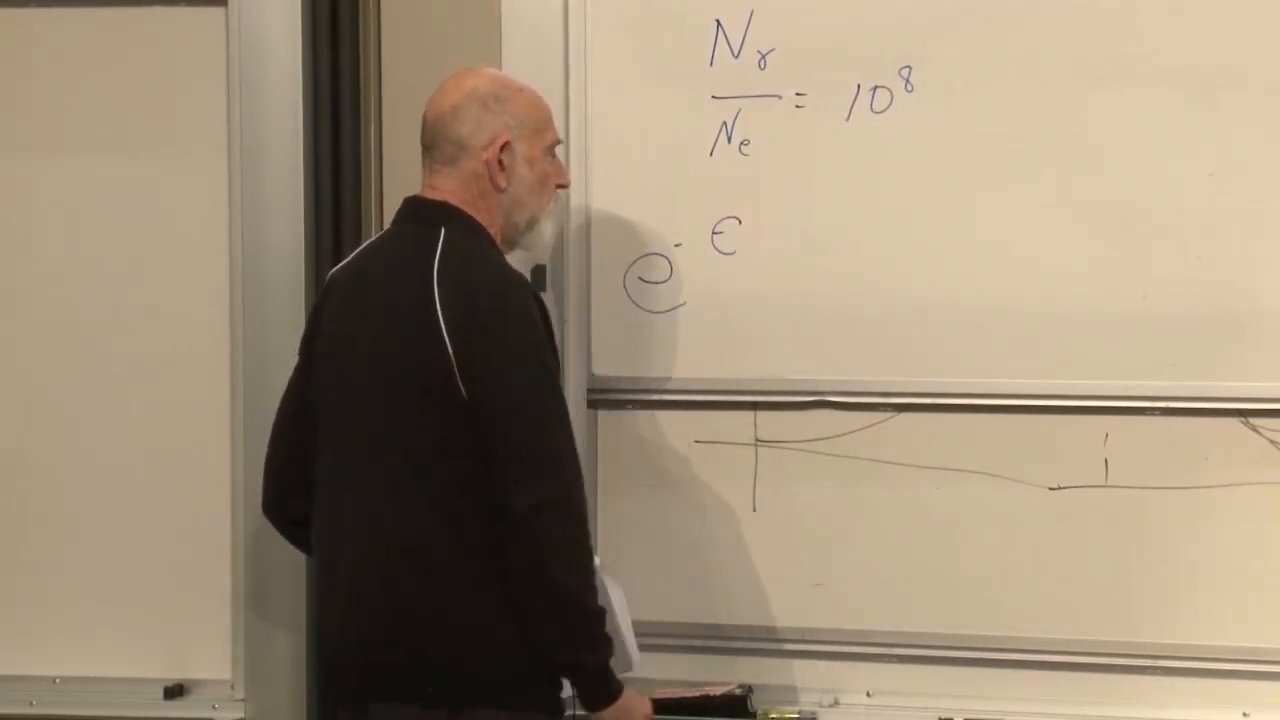
\includegraphics[width=0.82\textwidth]{lecture_07_figure_03.png}
\caption{На доске вводятся наблюдаемое отношение численностей \(N_\gamma/N_e=10^8\) и обозначение энергии фотона \(\epsilon\). Видно только начало экспоненты; полный множитель Больцмана следует из устного вывода.}
\label{fig:c07-boltzmann-board}
\lectureframe{01:06:10.631}
\end{figure}

Используемое здесь округлённое отношение численностей равно
\begin{equation}
\frac{N_\gamma}{N_e}\sim10^8.
\label{eq:c07-photon-electron-ratio}
\end{equation}
Его получают, сравнивая измеренную плотность фотонов реликтового микроволнового фона с содержанием обычного вещества. Для энергии фотона \(\epsilon\) высокоэнергетический хвост имеет больцмановский вид
\begin{equation}
P(\epsilon)\propto e^{-\epsilon/(k_BT)}.
\end{equation}
Поэтому число ионизующих фотонов, приходящееся на один атом, оценивается как
\begin{equation}
10^8 e^{-\chi_H/(k_BT)}.
\end{equation}
Ионизация остаётся эффективной, пока эта величина не упадёт до порядка единицы.

Логарифмирование даёт
\begin{equation}
\frac{\chi_H}{k_BT}
\sim
\ln 10^8
\simeq18.4,
\end{equation}
или, с требуемой здесь точностью,
\begin{equation}
k_BT\sim\frac{\chi_H}{20}.
\label{eq:c07-tail-estimate}
\end{equation}
Характерный фотон может иметь энергию далеко ниже порога, потому что для каждого атома достаточно одного ионизующего фотона из хвоста.

\begin{classroomqa}
\audiencequestion{Учитывает ли оценка по хвосту фотоны ровно на пороге или все фотоны выше него?}
\lecturerresponse{Она учитывает фотоны на пороге и выше него. Поскольку хвост убывает экспоненциально, основная часть этого интеграла приходится на энергии вблизи \(\chi_H\), так что простая экспоненциальная оценка даёт правильный порядок величины. \lecturetimestamp{01:08:39--01:08:54}}
\end{classroomqa}

\begin{classroomqa}
\audiencequestion{Было ли отношение \(N_\gamma/N_e\) при развязке тоже порядка \(10^8\)?}
\lecturerresponse{В использованном здесь приближении — да. От развязки назад, к существенно более горячим эпохам, расширение разрежает обе популяции одним и тем же объёмным множителем и не создаёт и не уничтожает достаточно много частиц ни одного из видов, чтобы изменить их отношение. При ещё более высоких температурах реакции рождения пар требуют иного учёта. \lecturetimestamp{01:08:54--01:09:57}}
\end{classroomqa}

\begin{classroomqa}
\audiencequestion{Вносят ли фотоны, испускаемые звёздами, заметный вклад в этот счёт?}
\lecturerresponse{Нет. Во время рекомбинации звёзд ещё не существовало, и даже сегодня их фотоны составляют лишь ничтожную долю популяции фотонов реликтового микроволнового фона. Отношение в уравнении~\eqref{eq:c07-photon-electron-ratio} относится к реликтовым тепловым фотонам. \lecturetimestamp{01:11:44--01:12:39}}
\end{classroomqa}

\begin{classroomqa}
\audiencequestion{Когда электроны рекомбинируют с протонами, должны ли испущенные фотоны оставить в спектре чёрного тела резкую водородную особенность?}
\lecturerresponse{Пока рассеяние и поглощение остаются быстрыми по сравнению с расширением, излучение непрерывно перерабатывается и остаётся близким к тепловому равновесию. При достаточно резком выходе из равновесия искажение могло бы сохраниться, но медленная рекомбинация, происходящая почти в равновесии, не позволяет большой изолированной линии заменить чернотельную форму. \lecturetimestamp{01:12:42--01:14:07}}
\end{classroomqa}

Получающаяся в аудитории оценка равна \(T_{\rm dec}\sim4\times10^3\,\mathrm{K}\). Непосредственный пересчёт \(\chi_H/20\) даёт несколько большее значение, что наводит на мысль, что эффективный знаменатель может быть ближе к \(40\). Это не противоречие; оно показывает грубость замены полного ионизационного баланса одним подсчётом по хвосту. Систематическое равновесное рассмотрение использует соотношение Саха,
\begin{equation}
\frac{x_e^2}{1-x_e}
=
\frac{1}{n_H}
\left(\frac{m_e k_BT}{2\pi\hbar^2}\right)^{3/2}
e^{-\chi_H/(k_BT)},
\label{eq:c07-saha}
\end{equation}
а затем — неравновесную кинетику рекомбинации. Грубый аргумент ценен тем, что выявляет доминирующий физический механизм: крошечное отношение числа барионов к числу фотонов задерживает устойчивое существование нейтральных атомов до температуры, гораздо меньшей, чем \(\chi_H/k_B\).

\section{Красное смещение поверхности последнего рассеяния}

При \(T_0\simeq3\,\mathrm{K}\) и \(T_{\rm dec}\sim4\times10^3\,\mathrm{K}\) уравнение~\eqref{eq:c07-decoupling-ratio} даёт
\begin{equation}
\boxed{
\frac{a_0}{a_{\rm dec}}
\sim
\frac{T_{\rm dec}}{T_0}
\sim10^3
}.
\label{eq:c07-decoupling-expansion}
\end{equation}
Эквивалентно, красное смещение последнего рассеяния имеет порядок \(10^3\). До этой эпохи ионизованная плазма была непрозрачной; после неё фотоны распространялись почти свободно.

Это тепловое событие произошло всего через несколько сотен тысяч лет после начала горячего расширения; в обсуждении обычно называют величину порядка \(380{,}000\) лет. Этот промежуток ничтожен по сравнению с последующим возрастом Вселенной. Со времени развязки длины выросли примерно в \(10^3\), а комовинговые элементы объёма — примерно в \(10^9\).

Развязка — одна из тепловых вех, а не единственное событие в промежуточной истории. Образование галактик, звёзд и чёрных дыр происходит позже, но здесь это оставлено в стороне, чтобы можно было ясно проследить тепловые вехи назад.

Смотреть вдаль — значит смотреть назад. Ближние оболочки показывают недавние эпохи; более далёкие — более ранние. Наш прошлый световой конус в конце концов пересекает эпоху рекомбинации, и его пересечение с этой эпохой и есть поверхность последнего рассеяния. Более раннее электромагнитное излучение многократно рассеивалось на свободных зарядах и не могло прийти к нам напрямую.

\begin{figure}[htbp]
\centering
\begin{coursefitfigure}
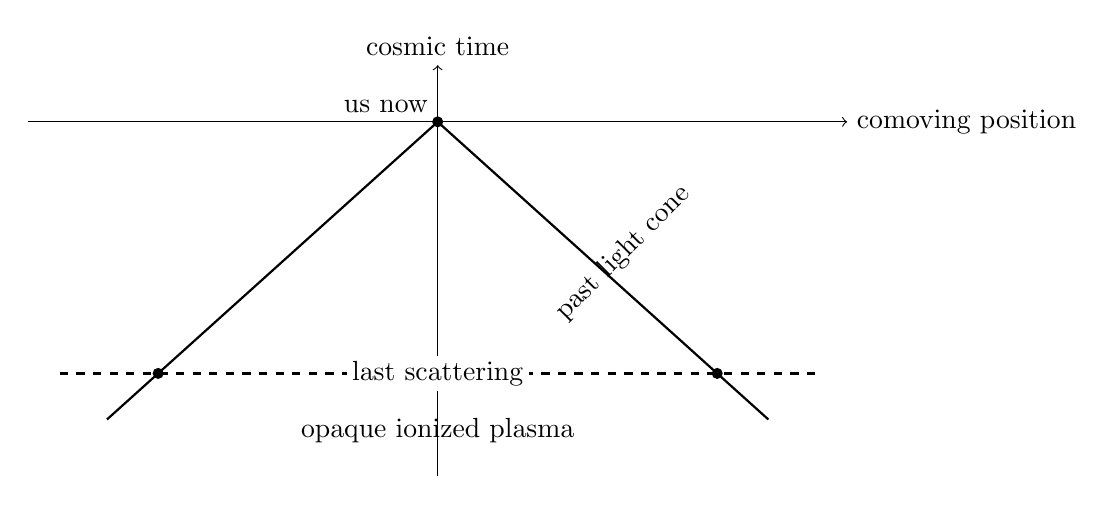
\begin{tikzpicture}[x=1.0cm,y=0.9cm]
\draw[->] (0,0)--(0,5.8) node[above] {cosmic time};
\draw[->] (-5.2,5.0)--(5.2,5.0) node[right] {comoving position};
\draw[thick] (0,5.0)--(-4.2,0.8);
\draw[thick] (0,5.0)--(4.2,0.8);
\draw[thick,dashed] (-4.8,1.45)--(4.8,1.45);
\fill (0,5.0) circle (2pt) node[above left] {us now};
\fill (-3.55,1.45) circle (2pt);
\fill (3.55,1.45) circle (2pt);
\node[fill=white,inner sep=2pt] at (0,1.45) {last scattering};
\node at (0,0.65) {opaque ionized plasma};
\node[rotate=45] at (2.35,3.15) {past light cone};
\end{tikzpicture}
\end{coursefitfigure}
\caption{Электромагнитные наблюдения простираются назад вдоль прошлого светового конуса лишь до поверхности последнего рассеяния. Более ранние фотоны многократно рассеивались ионизованной плазмой.}
\label{fig:c07-last-scattering}
\end{figure}

\begin{classroomqa}
\audiencequestion{Означает ли развязка конец всех возможных наблюдений более ранних эпох?}
\lecturerresponse{Она завершает прямое электромагнитное наблюдение, потому что плазма была непрозрачна для фотонов. Более слабо взаимодействующие вестники могли уйти раньше: реликтовые нейтрино в принципе зондируют более глубокий слой, а гравитационное излучение могло бы нести информацию из ещё более ранних эпох. Поэтому значительная часть наших знаний о том, что было до последнего рассеяния, косвенна, но не произвольна. \lecturetimestamp{01:32:27--01:36:31}}
\end{classroomqa}

\begin{classroomqa}
\audiencequestion{Каково было абсолютное значение \(a\) в начале, и обязательно ли Вселенная была крошечным конечным объектом?}
\lecturerresponse{В плоском пространстве инвариантный смысл имеют только отношения масштабных факторов; нормировка \(a\) произвольна. Пространственный срез отрицательной кривизны тоже может быть бесконечным. Замкнутая вселенная \(k=+1\) имеет конечный радиус кривизны, но наблюдения всё равно определяют отношения расширения, а не некоторый известный первичный размер. Горячий Большой взрыв сам по себе не означает, что всё пространство было крошечным шаром. \lecturetimestamp{01:30:05--01:32:22}}
\end{classroomqa}

\begin{classroomqa}
\audiencequestion{Поскольку реликтовое излучение старше галактик, говорит ли его наблюдение нам о том, существуют ли сегодня галактики за пределами нашей наблюдаемой области?}
\lecturerresponse{Нет. Оно показывает далёкую область такой, какой она была при развязке, а не такой, какова она сегодня. Свет от современных галактик на достаточно большом расстоянии не успел до нас дойти. В пользу того, что за нашим горизонтом галактики продолжают существовать, говорят наблюдаемая крупномасштабная однородность и отсутствие видимого края, а не прямой обзор, обеспечиваемый реликтовым излучением. \lecturetimestamp{01:59:01--02:00:58}}
\end{classroomqa}

Получающаяся временная шкала идёт назад от настоящего через образование галактик и развязку к равенству материи--излучения. Ещё раньше уменьшение масштабного фактора означает рост температуры и появление новых видов частиц.

\section{Равенство материи--излучения}

Если двигаться назад дальше развязки, появляется ещё одна веха. Нерелятивистская материя и излучение разрежаются по-разному:
\begin{equation}
\rho_m\propto a^{-3},
\qquad
\rho_r\propto a^{-4},
\qquad
\frac{\rho_m}{\rho_r}\propto a.
\label{eq:c07-equality-scaling}
\end{equation}
На поздних стадиях доминирует материя, но при достаточно малом \(a\) неизбежно доминирует излучение. Соответственно закон расширения меняется от поведения эпохи материи \(a\propto t^{2/3}\) к поведению эпохи излучения \(a\propto t^{1/2}\).

Намеренно грубая оценка начинается с \(10^8\) фотонов на протон, характерной энергии фотона реликтового излучения \(10^{-4}\,\mathrm{eV}\) и энергии покоя протона \(10^9\,\mathrm{eV}\). Если пренебречь тёмной материей, получаем
\begin{equation}
\left(\frac{\rho_m}{\rho_r}\right)_0
\sim
\frac{10^9}{10^8\,10^{-4}}
\sim10^5.
\end{equation}
Затем это рассуждение приходится поправить: тёмная материя даёт существенно больший вклад в массу, чем светящиеся барионы, повышая округлённую оценку до \(10^6\). В рамках этой арифметики уравнение~\eqref{eq:c07-equality-scaling} помещает равенство в точку
\begin{equation}
\frac{a_{\rm eq}}{a_0}\sim10^{-6},
\qquad
\frac{T_{\rm eq}}{T_0}\sim10^6.
\label{eq:c07-equality-estimate}
\end{equation}
Это учебные оценки, задающие масштаб, а не точная подгонка космологических параметров. Их цель — показать, как разные степени \(a\) определяют положение последовательных тепловых эпох.

Эпоха доминирования излучения лежит за электромагнитной стеной последнего рассеяния, но её существование следует из измеренных плотностей на поздних стадиях и известных законов масштабирования. При переходе к ещё более высокой температуре предположение о том, что числа протонов, электронов и фотонов по отдельности фиксированы, в конце концов перестаёт быть верным, поскольку энергичные столкновения начинают порождать массивные пары частица--античастица.

\begin{classroomqa}
\audiencequestion{Включает ли утверждение о сохранении числа фотонов и протонов звёздный свет и сколь угодно высокие температуры?}
\lecturerresponse{Нет. Оно относится к реликтовой популяции фотонов на интервале, где реакции, меняющие их число, неэффективны. Звёздный свет возник позже, и его вклад в число фотонов пренебрежимо мал. При достаточно высокой температуре рождение пар меняет состав частиц, и отдельное сохранение числа перестаёт выполняться. Сама рекомбинация добавляет не более примерно одного фотона на электрон, то есть лишь одну долю в \(10^8\) от уже существующей реликтовой популяции. \lecturetimestamp{01:26:24--01:27:40}}
\end{classroomqa}

\section{Рождение пар и почти симметричный суп}

При температуре порядка
\begin{equation}
T\sim10^{10}\,\mathrm{K},
\qquad
\frac{a_0}{a}\sim10^{14},
\end{equation}
характерная энергия фотона составляет около мегаэлектрон-вольта, что сравнимо с масштабом энергии покоя, необходимым для образования пары электрон--позитрон. Тогда два фотона могут вступать в реакцию
\begin{equation}
\gamma+\gamma
\longleftrightarrow
e^-+e^+.
\label{eq:c07-pair-reaction}
\end{equation}
Точный порог зависит от кинематики столкновения, но энергия покоя электрона, \(m_ec^2\), задаёт соответствующий масштаб.

Рождение пар и аннигиляция быстро уравновешивают друг друга. Если пар слишком мало, столкновения фотонов пополняют их; если их слишком много, аннигиляция возвращает их энергию фотонам. Поэтому количества фотонов, электронов и позитронов определяются температурой и все имеют сравнимый порядок величины в релятивистской плазме. Они уже не сохраняют простой памяти о своих позднейших числах.

\begin{classroomqa}
\audiencequestion{Как эта наполненная парами плазма может оставаться электрически нейтральной, если уже есть электроны, нужные для компенсации протонов?}
\lecturerresponse{Каждая реакция создаёт один отрицательный и один положительный заряд, так что пары не добавляют суммарного заряда. Они представляют собой огромную почти симметричную популяцию, наложенную на крошечный избыток электронов. Отдельные электроны неразличимы; только разность \(N_{e^-}-N_{e^+}\) хранит информацию о заряде, необходимом для компенсации протонов. \lecturetimestamp{01:42:31--01:43:14}}
\end{classroomqa}

Реакции с парами меняют сумму, но сохраняют разность:
\begin{equation}
N_{e^-}+N_{e^+}\quad\hbox{changes},
\qquad
N_{e^-}-N_{e^+}=\hbox{constant}.
\label{eq:c07-pair-invariants}
\end{equation}
В горячем супе \(N_{e^-}+N_{e^+}\) имеет тот же порядок, что и \(N_\gamma\), тогда как сохраняющийся избыток имеет тот же порядок, что и гораздо меньшее число протонов. Поэтому округлённое отношение равно
\begin{equation}
\boxed{
\frac{N_{e^-}-N_{e^+}}
{N_{e^-}+N_{e^+}}
\sim10^{-8}
}.
\label{eq:c07-asymmetry}
\end{equation}
На каждые \(10^8\) электрон--позитронных пар приходился примерно один лишний электрон.

Это переворачивает исходный вопрос. Поразителен не просто тот факт, что фотонов много. При высокой температуре фотоны и пары естественным образом имеют сравнимые количества. Загадка состоит в том, почему популяции отрицательных и положительных частиц вообще различаются и почему их относительное различие мало, а не в точности равно нулю и не имеет порядка единицы. Симметричное начальное состояние и симметричное рождение пар не дали бы никакого избытка. Микроскопическое происхождение ненулевой асимметрии — вот проблема, переходящая на следующий этап обсуждения.

При температурах ещё на два или три порядка выше структуру протона уже нельзя игнорировать. Столкновения рождают кварки и антикварки, а протоны распадаются на свои составляющие; фотоны, лептоны, кварки, антикварки, глюоны и любые достаточно лёгкие тёмные виды частиц образуют более горячую плазму. Энергия вакуума там динамически пренебрежимо мала, потому что плотность излучения растёт как \(a^{-4}\).

Соответствующий избыток кварков связан с избытком электронов общей электрической нейтральностью. Барион составляют три валентных кварка, поэтому при подсчёте возникают обычные коэффициенты, но оставшаяся барионная материя и оставшиеся электроны не являются независимыми дисбалансами заряда. Их общая малость — реликт ранней Вселенной.

Теперь снова проследим эволюцию электрон--позитронной плазмы вперёд. Когда температура падает ниже масштаба рождения пар, аннигиляция продолжается, тогда как обратная реакция становится редкой. Почти каждый электрон находит позитрон, энергия пары переходит в излучение, и остаётся лишь крошечная несокомпенсированная популяция электронов. Окружающая нас материя — это этот остаточный дисбаланс, а не типичный образец некогда огромной популяции пар.

\begin{classroomqa}
\audiencequestion{Что происходило с протонами в эпоху аннигиляции электрон--позитронных пар?}
\lecturerresponse{На этом этапе температура была достаточно высокой, чтобы рождать электронные пары, но ещё недостаточно высокой, чтобы рождать в большом числе протон--антипротонные пары или разлагать протоны на кварки. Поэтому популяция протонов была мала, но сохранялась, и нейтральность требовала \(N_{e^-}-N_{e^+}\simeq N_p\). \lecturetimestamp{01:55:35--01:56:53}}
\end{classroomqa}

Во всей видимой Вселенной, по-видимому, знак избытка вещества один и тот же. В качестве учебного довода приводится отсутствие антиядер в космических лучах: вторичные столкновения могут иногда рождать антипротоны, но от антигалактики ожидалось бы поступление сложных антиядер. Это наблюдательный аргумент уровня лекции, а не утверждение о том, что области за пределами наблюдаемого горизонта были исследованы.

\begin{classroomqa}
\audiencequestion{Может ли наблюдаемый избыток вещества быть локальной флуктуацией, а за пределами того, что мы видим, существовать области антивещества?}
\lecturerresponse{Одинаковый знак во всём огромном наблюдаемом объёме слишком согласован, чтобы быть случайной флуктуацией. Это требует динамического объяснения. Однако за пределами наблюдаемой области прямые свидетельства недоступны; переход к иному домену нельзя исключить, просто пытаясь заглянуть дальше, чем свет успел до нас дойти. \lecturetimestamp{01:56:57--01:58:47}}
\end{classroomqa}

\begin{classroomqa}
\audiencequestion{Является ли объяснение вещества--антивещества уже точной количественной теорией, и происходит ли объединение взаимодействий при этой температуре?}
\lecturerresponse{Существует качественная теория того, как может возникнуть малая асимметрия, но округлённое значение \(10^{-8}\) здесь не выводится из единственной микроскопической модели. Объединение взаимодействий происходит при температурах намного выше, чем в эпоху электронных пар. Оба вопроса требуют физики за пределами нынешних тепловых вех. \lecturetimestamp{01:51:36--01:52:24}}
\end{classroomqa}

\section{Что нужно иметь в виду дальше}

Тепловую историю определяют скорости процессов и пороги. Быстрое рассеяние устанавливает общую температуру; образование нейтральных атомов устраняет рассеивающие частицы; затем однородное расширение смещает замороженный планковский спектр в красную сторону, не разрушая его формы. Поэтому КМФ служит и термометром излучения, и видимой поверхностью, отмечающей конец прямого электромагнитного доступа к более ранней плазме.

Избыток фотонов делает рекомбинацию проблемой хвоста, а не проблемой средней энергии. Масштаб \(T_{\rm dec}/T_0\sim10^3\) определяет положение последнего рассеяния, тогда как различные законы разбавления для вещества и излучения указывают на более раннюю эпоху равенства. При ещё более высокой температуре рождение пар стирает память об общем числе электронов и позитронов, но сохраняет их крошечную разность. Эта остаточная асимметрия, отражённая и в барионном секторе, — то необъяснённое исходное данное, с которым должно будет иметь дело следующее исследование.